\documentclass[11pt]{article}

\usepackage[a4paper]{geometry}
\usepackage{amsmath, amsthm, amssymb, amsthm, graphicx, hyperref}
\renewcommand\labelenumi{\alph{enumi}.}
\renewcommand\labelenumii{\roman{enumii}.}
\renewcommand\labelitemi{--}
\setlength\parindent{0pt}



\title{1B - Computer Graphics and Image Processing\\
Supervision 2}
\author{Raahil Shah\\
\texttt{rds46@cam.ac.uk}}

\begin{document}

\maketitle

\section{Matrices}
Give as many reasons as possible why we use matrices to represent transformations. Explain why we use homogeneous co-ordinates. 

Reasons to use matrices to represent transformations:
\begin{itemize}
	\item Since we use vectors to represent both our 3D and 2D coordinates, linear transformations on vectors can be conveniently represented as matrices.
	\item Transformations can be combined into a single transformation with matrix algebra (multiplying individual transformation matrices).
	\item Applying matrix transformations to vectors is highly parallelizable and so can be performed quickly on SIMD processors like GPUs. 
	\item Transformations become pluggable in the sense that changing a transformation in a series of transformations entails just replacing the transformation matrix in the multiplication. 
	\item Transformations can be reversed by computing the inverse of the transformation matrix. 
\end{itemize}

Homogeneous coordinates are using in computer graphics because they allow us to represent the translation operation as a matrix, allowing us to use the same hardware optimized for parallel matrix operations (of rotation, scaling etc.) for translation as well. Further, in homogeneous coordinates each Cartesian coordinate can be represented by an infinite number of homogeneous coordinates and we can define a representation for a point at infinity. 


\section{Bezier cubics}
Derive the conditions necessary for two Bezier curves to join with 
\begin{itemize}
	\item Just $C_0$-continuity
	\item $C_1$-continuity
	\item $C_2$-continuity. 
\end{itemize}

Given two Bezier curves:
\begin{align*}
	p(t) &= (1 - t)^3 P_0 + 3t(1 - t^2)P_1 + 3t^2(1 - t)P_2 + t^2 P_3 \\
	q(t) &= (1 - t)^3 Q_0 + 3t(1 - t^2)Q_1 + 3t^2(1 - t)Q_2 + t^2 Q_3
\end{align*}

Without loss of generality we join the curves at the $P_3$ and $Q_0$.
We can derive the continuity conditions as:
\begin{description}
	\item[C$_0$ continuity] requires \\
	Continuity in position:
	\[
	P_3 = Q_0 
	\]
	\item[C$_1$ continuity] requires \\
	Continuity in position: 
	\[
	P_3 = Q_0 
	\]
	Continuity in first derivative:
	\begin{align*}
		p'(1) &= q'(0) \\
		p'(1) &= 3(P_3 - P_2) \\
		q'(0) &= 3(Q_1 - Q_0) \\
		\implies P_3 - P_2 &= Q_1 - Q_0
	\end{align*}
	\item[C$_2$ continuity] requires \\
	Continuity in position: 
	\[
	P_3 = Q_0 
	\]
	Continuity in first derivative:
	\[
		P_3 - P_2 = Q_1 - Q_0
	\]
	Continuity in second derivative:
	\begin{align*}
		p''(1) &= q''(0) \\
		p''(1) &= 6P_1 - 12P_2 + 6P_3 \\
		q''(0) &= 6Q_0​­ - 12Q_​1 + 6Q_2 \\
		\implies P_1 - 2P_2 + P_3 &= Q_0 - 2Q_1 + Q_2
	\end{align*}



\end{description}

What would be difficult about getting three Bezier curves to join in sequence with C2-continuity at the two joins?

Given the first two curves $p$ and $q$, the C$_2$ continuity condition between p and $q$ fixes:
\begin{align*}
	Q_0 &= P_3 \\
	Q_1 &= 2P_3 - P_2 \\
	Q_2 &= P_1 - 4P_2 + 4P_3
\end{align*}
allowing us to chose only the $Q_3$ endpoint for our curve which must be the same as the start $R_0$ of the third curve $r$. For $r$ we will also have 3 of its point fixed by $q$ allowing us to chose only the end point. So not all pairs of Bezier curves $p$ and $r$ can be joined together by a third Bezier curve $q$ under C$_2$ continuity. 

\section{Curves}
\begin{enumerate}
	\item Implement the Midpoint circle drawing algorithm for integer radius and integer center location. 
	Hints: 
	\begin{enumerate}
		\item Implement the algorithm for one octant, centered on the origin, then draw the other octants by manipulating the co-ordinates of the drawn point: (x,y), (-x,y), (y,x), (y,-x), etc.
		\item Implement the algorithm for a circle centered on the origin and then simply offset the pixel that is drawn by the coordinates of the actual center.
	\end{enumerate}
	\begin{figure}[!htbp]
		\begin{center}
			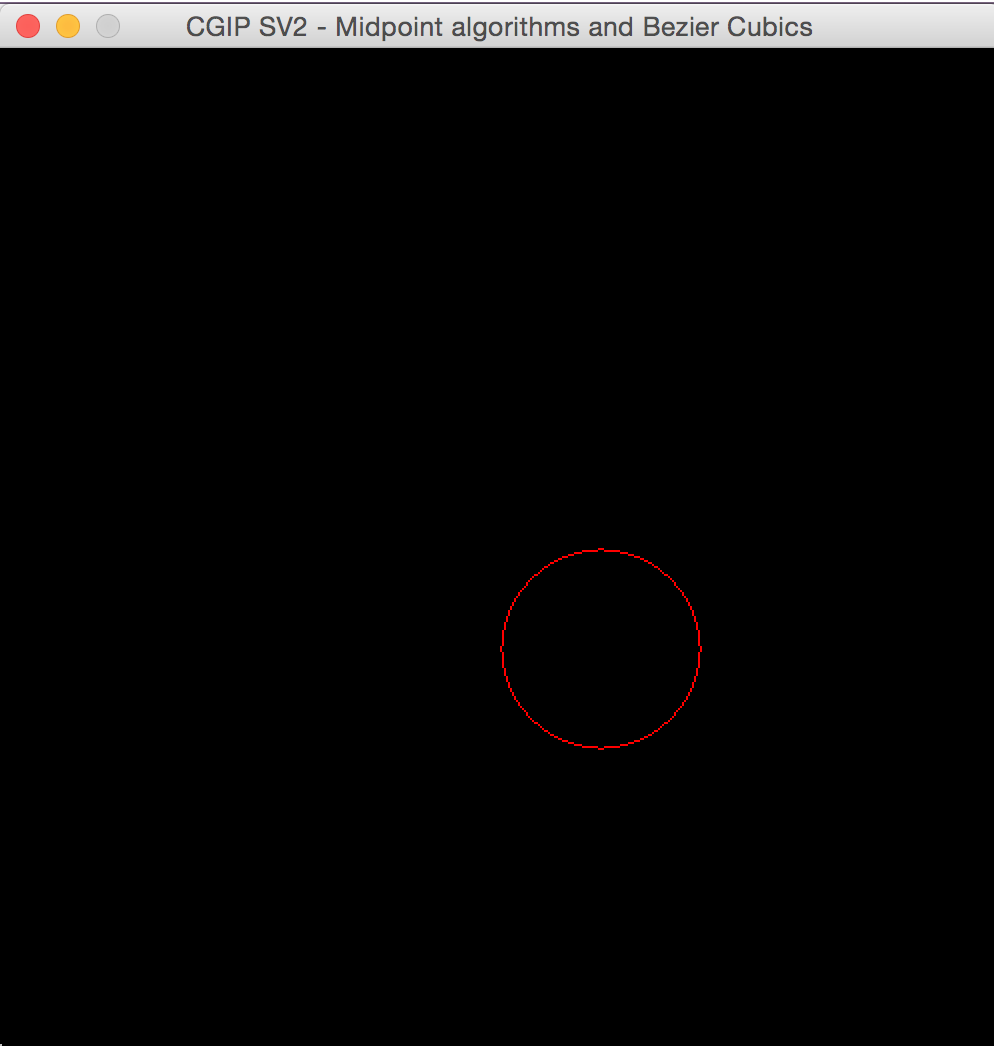
\includegraphics[scale=0.4]{circle}
		\end{center}
		\caption{Circle drawing with the midpoint algorithm.}
	\end{figure}

	\item 
	Write the Bezier adaptive algorithm, using your Midpoint line drawing to draw the lines. To test this on a pixel grid of size HxW, try the Bezier curve specified by the four points: (1,1), (2H,1), (-H,W-1), (H-1,W-1). Draw the same Bezier curve at five different tolerances: 33, 10, 3.3, 1, 0.33 pixels.
	\begin{figure}[!htbp]
		\begin{center}
			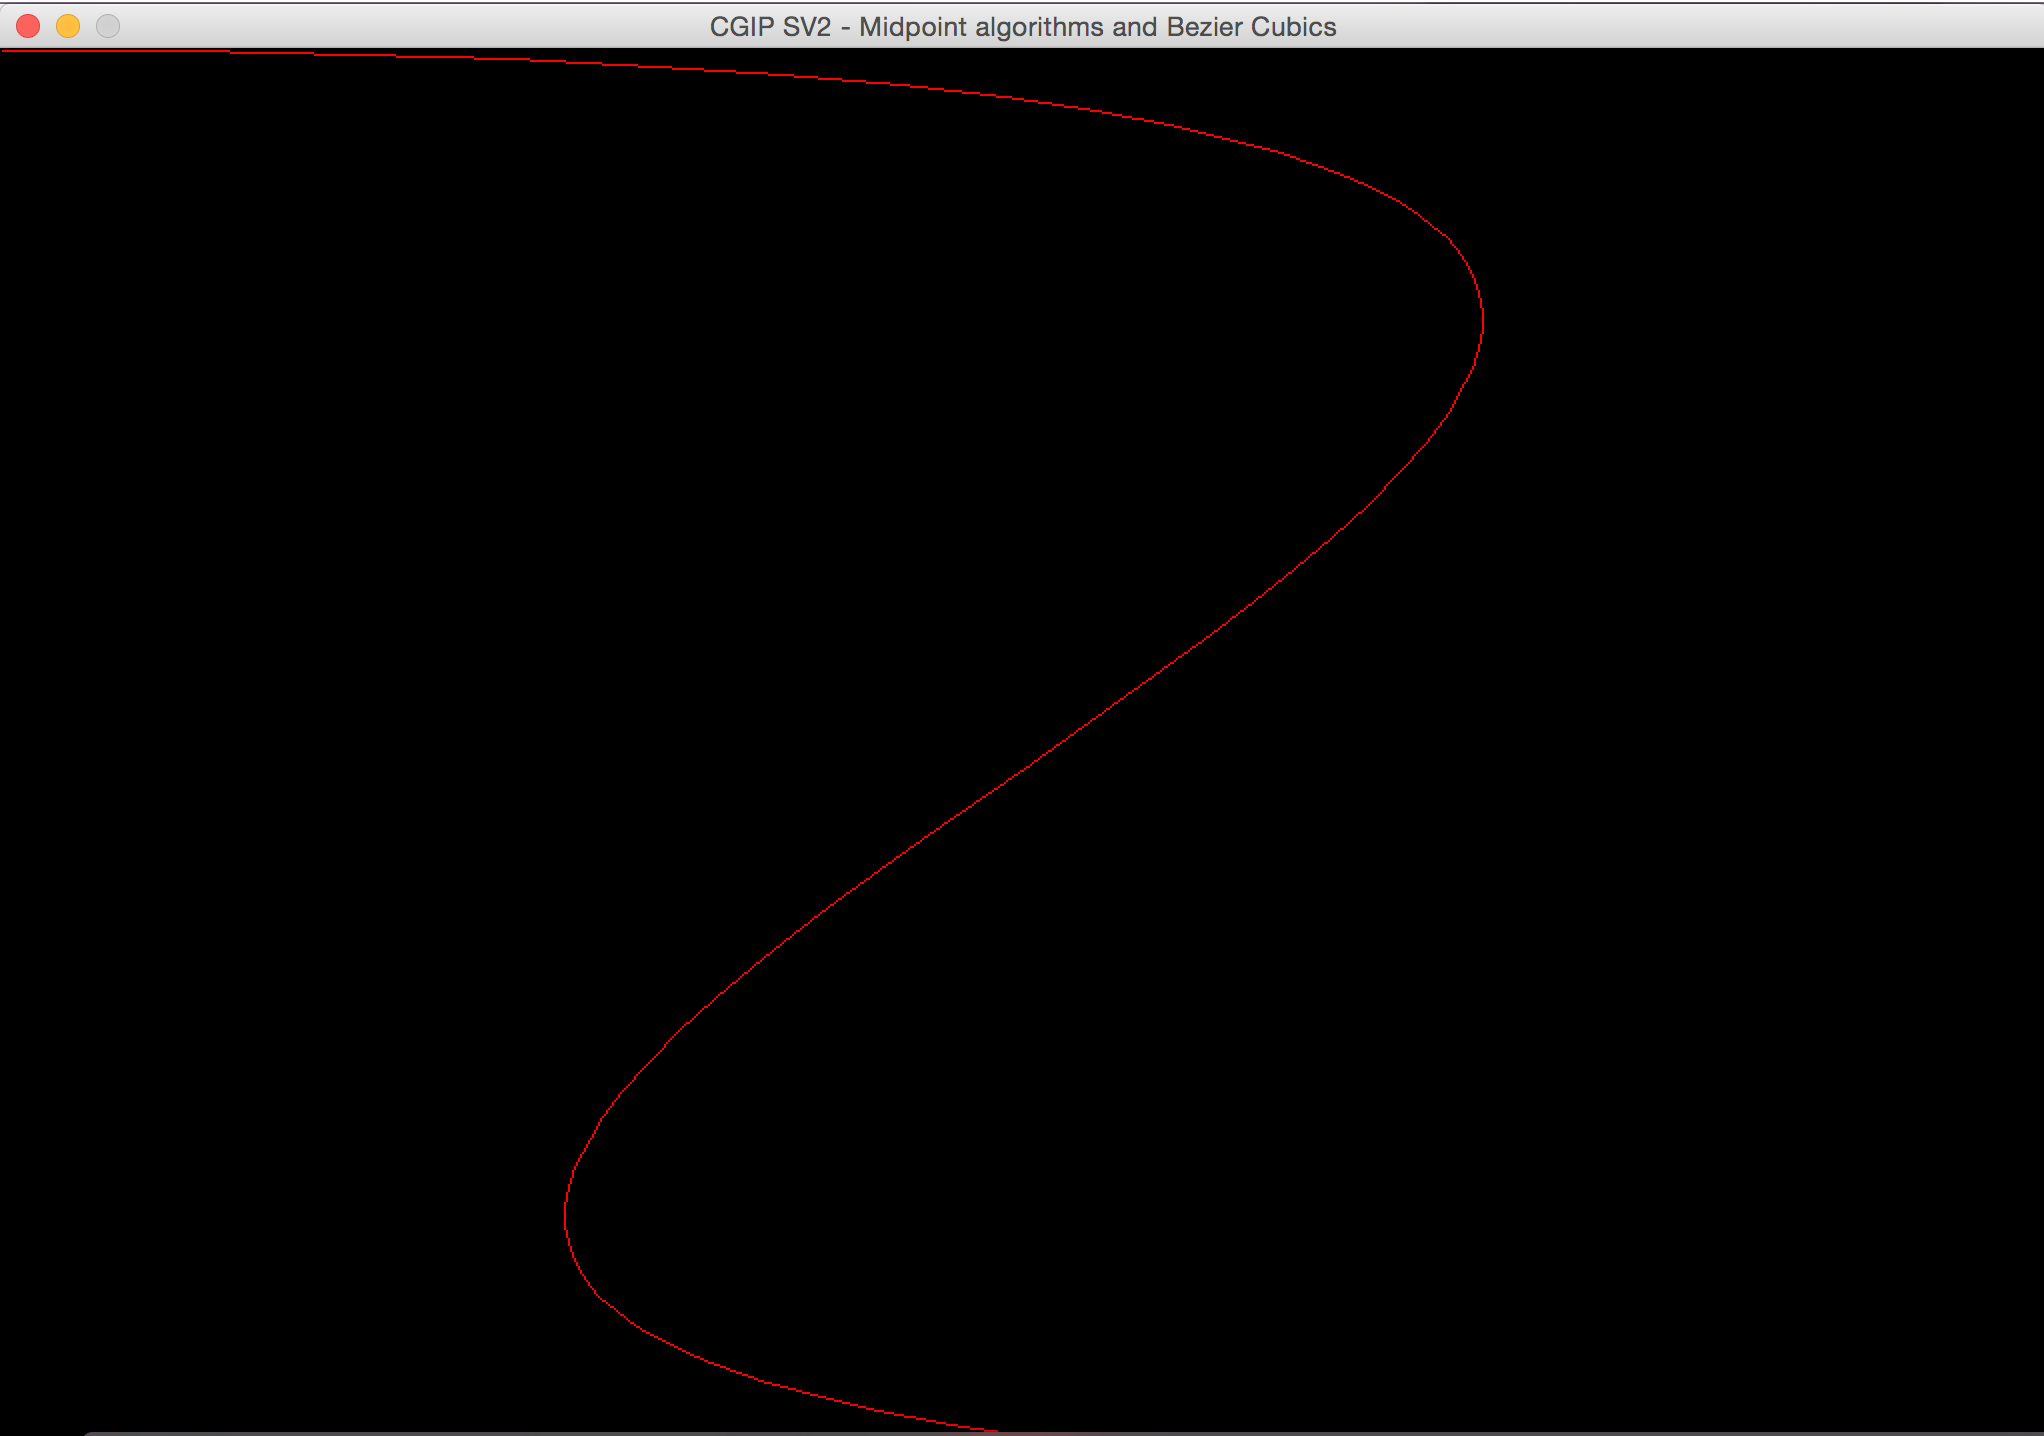
\includegraphics[scale=0.4]{bezier}
		\end{center}
		\caption{Given Bezier cubic drawn with tolerance 0.33 and using midpoint line drawing.}
	\end{figure}
	\item Draw something interesting!
	\pagebreak
	\begin{figure}[!htbp]
		\begin{center}
			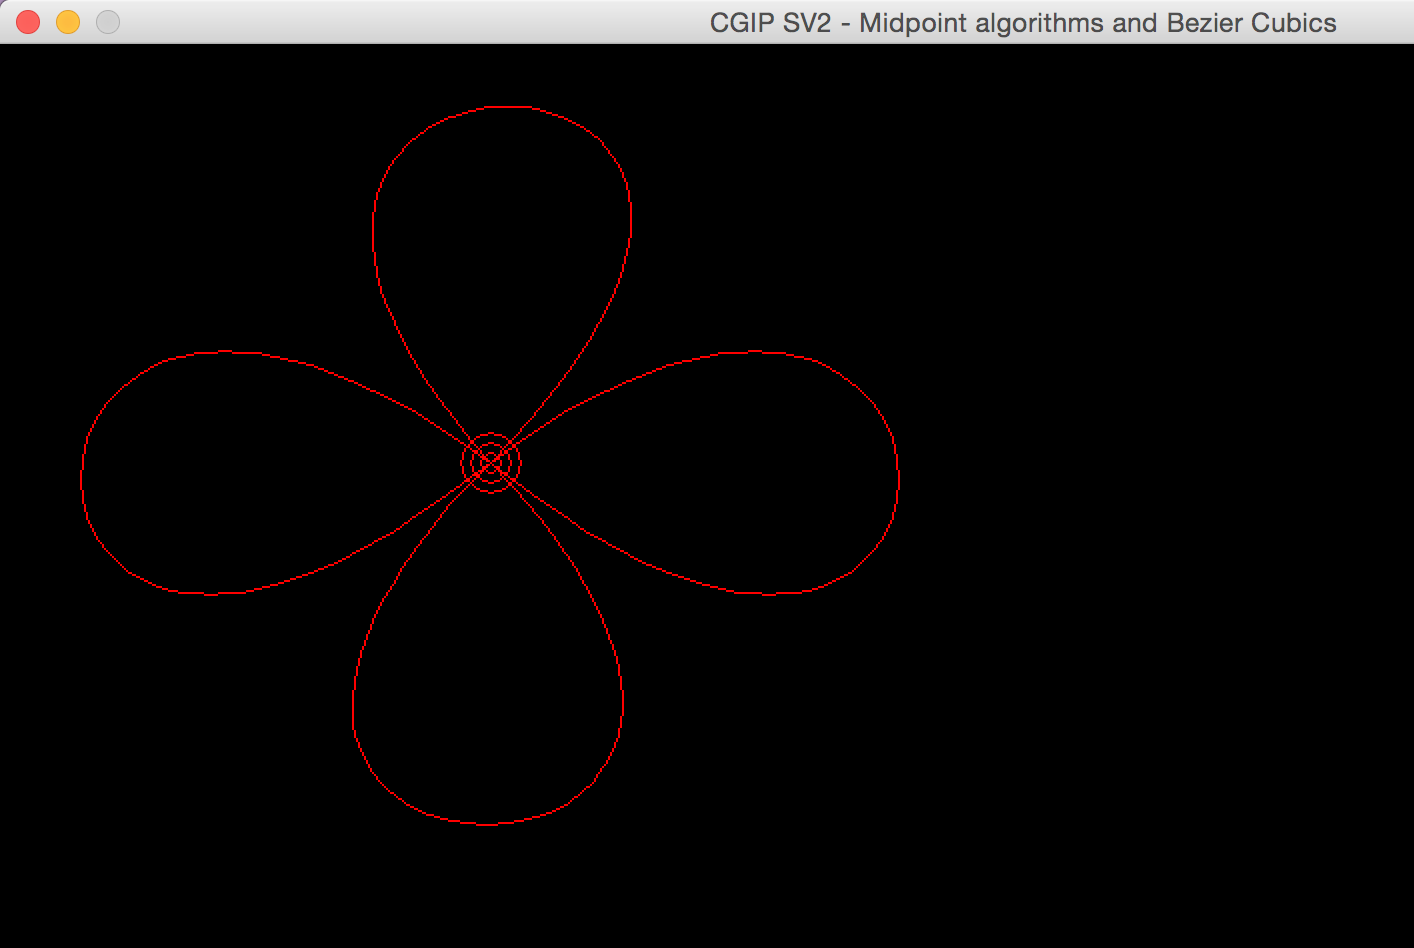
\includegraphics[scale=0.6]{flower}
		\end{center}
		\caption{Four petaled flower using Bezier curves and circles.}
	\end{figure}

	The code for the algorithms is up on: 
	\url{https://github.com/raahilshah/CGIP/tree/master/src/uk/ac/cam/rds46/cgip/sv2}
\end{enumerate}



\end{document}